%
% PROJECT: <ETD> Electronic Thesis and Dissertation Initiative
%   TITLE: LaTeX report template for ETDs in LaTeX
%  AUTHOR: Neill Kipp, nkipp@vt.edu
%     URL: http://etd.vt.edu/latex/
% SAVE AS: etd.tex
% REVISED: September 6, 1997 [GMc 8/30/10]
% 

% Instructions: Remove the data from this document and replace it with your own,
% keeping the style and formatting information intact.  More instructions
% appear on the Web site listed above.
\documentclass[12pt]{report}

\setlength{\textwidth}{6.5in}
\setlength{\textheight}{8.5in}
\setlength{\evensidemargin}{0in}
\setlength{\oddsidemargin}{0in}
\setlength{\topmargin}{0in}

\setlength{\parindent}{0pt}
\setlength{\parskip}{0.1in}

% Uncomment for double-spaced document.
% \renewcommand{\baselinestretch}{2}

% \usepackage{epsf}
\usepackage{times}
\usepackage{epsfig}
\usepackage{wrapfig}
\usepackage{multicol}
\usepackage{soul}
\usepackage{multirow}
\usepackage{color}
\usepackage{psfrag}
\usepackage[linesnumbered,ruled,commentsnumbered]{algorithm2e}
\usepackage{subfigure}
\usepackage{booktabs}
\usepackage{float}
\usepackage{url}
\usepackage{path}
\usepackage{caption}
\usepackage{courier}
\usepackage{listings}
\usepackage{pifont}
\usepackage{graphicx}
\usepackage{comment} 
\usepackage{titlesec}
\setcounter{secnumdepth}{4}
\usepackage{epstopdf}
\DeclareGraphicsExtensions{.eps}

\usepackage{float}
\usepackage{lipsum}
\usepackage{pdflscape}
\usepackage{afterpage}
\usepackage{pbox}
\usepackage{fixltx2e}
\usepackage{tocbibind}

\newcommand{\otoprule}{\midrule[\heavyrulewidth]}
\newcommand\mvspace[1][10pt]{\rule[\normalbaselineskip]{0pt}{#1}}

\newcommand{\cb}{\textcolor{blue}}

%% font definitions
%% fixed
\newenvironment{fixedtt}{\fontfamily{lmtt}\selectfont}{\par}
\DeclareTextFontCommand{\fixed}{\fixedtt\small}
\DeclareTextFontCommand{\fixedns}{\fixedtt}     % no resize
%% sans
\newenvironment{sanstt}{\fontfamily{phv}\selectfont\small}{\par}
\DeclareTextFontCommand{\sans}{\sanstt}
\newenvironment{sanstts}{\fontfamily{phv}\selectfont\smaller}{\par}
\DeclareTextFontCommand{\sanss}{\sanstts}

\usepackage{hyperref}
\renewcommand{\sectionautorefname}{\S}
\renewcommand{\subsectionautorefname}{\S}
\renewcommand{\subsubsectionautorefname}{\S}

%% source code styles
\lstset{
	basicstyle=\footnotesize\ttfamily,
	keywordstyle=\bfseries,
	extendedchars=true,
	breaklines=true,
	frame=lines,
	morekeywords={name,kernel,input,output,workdir,tasks}
}

%% table style
\renewcommand{\arraystretch}{1.1}

\begin{document}

\thispagestyle{empty}
\pagenumbering{roman}
\begin{center}

% TITLE
{\Large 
\bf{Interim Report --- CS 5604 Information Storage and Retrieval}\\\vspace{.1in}
\bf{\smaller CLA Team, Fall 2016}
}

\vfill

%Hyogi Sim

\vfill

%Thesis submitted to the Faculty of the \\
%Virginia Polytechnic Institute and State University \\
%in partial fulfillment of the requirements for the degree of

\vfill

{\bf CLA Team:}\\\vspace{.05in}
Saurabh Chakravarty\\
Mahesh Narayanamurthi\\
Hyogi Sim\\
\fixed{\{saurabc,maheshnm,hyogi\}@vt.edu}

\vfill

{\bf Project Advisor:}\\\vspace{.05in}
Prof. Edward A. Fox

\vfill

%%% TODO: we need to add the exact date.
September 20, 2016 \\
Blacksburg, Virginia

\vfill

Keywords: Text Classification, Information Retrieval, Information Storage
%\\
%Copyright \copyright 2014, Hyogi Sim

\end{center}

\pagebreak

\thispagestyle{empty}
\begin{center}

{\large
\bf{Interim Report --- CS 5604 Information Storage and Retrieval}
}

\vfill

{2016 Fall CLA Team}

\vfill

(ABSTRACT)

\vfill

\end{center}

%Document classification is a technique that algorithmically categorizes
%documents into a fixed set of categories.

In this term project, we aim to design and develop a document classification technique
that can complement the outcomes from the previous semesters.
Particularly, our design is focused on improving the following aspects, in
classifying the huge tweet collections into predefined categories.
First, the result of the classification should be reliable so they can be
practically utilized in decision makings.
To this end, we plan to achieve higher accuracy, by exploring and adopting the
state-of-the-art algorithms, than the previous classification techniques
provide.
In addition, an intelligent spam filtering technique will also be studied and developed.
Second, the classification system should perform in a scalable manner.
The amount of data that data analysis softwares need to ingest is
increasing unprecedentedly, and, therefore, it is crucial for such softwares to
provide deterministic and scalable performance for effectively supporting
decision making processes.
To achieve such scalability with respect to the increasing amount of the data,
our classification software will attentively orchestrate the I/O behaviors of
individual worker threads by considering the underlying system framework.

This interim report clarifies the problem that we address along with our
project goals, and summarizes related theories and practical techniques,
%including previous achievements in this course.
We then lastly provide our concrete execution plans.
%and lastly present our preliminary results.



\vfill

% GRANT INFORMATION

%That this work received support from the Southeastern Universities
%Research Association (SURA) ``Monticello Library Project'' is purely
%coincidental.

\pagebreak

% Dedication and Acknowledgments are both optional
%\chapter*{Dedication}
%\input{dedication}
% \chapter*{Acknowledgments}
% \input{ack}

\tableofcontents
\pagebreak

\listoffigures
\pagebreak

\listoftables
\pagebreak

\pagenumbering{arabic}
\pagestyle{myheadings}

\chapter{Introduction}

In this chapter, we describe the classification problem that we will address in our term project (\autoref{sec:problemstatement}), we state the assumptions with which we will be working and give a brief overview of the strategy that we will follow, details of which can be found in (\autoref{sec:design}).

\begin{figure}[tbh!]
\centering
 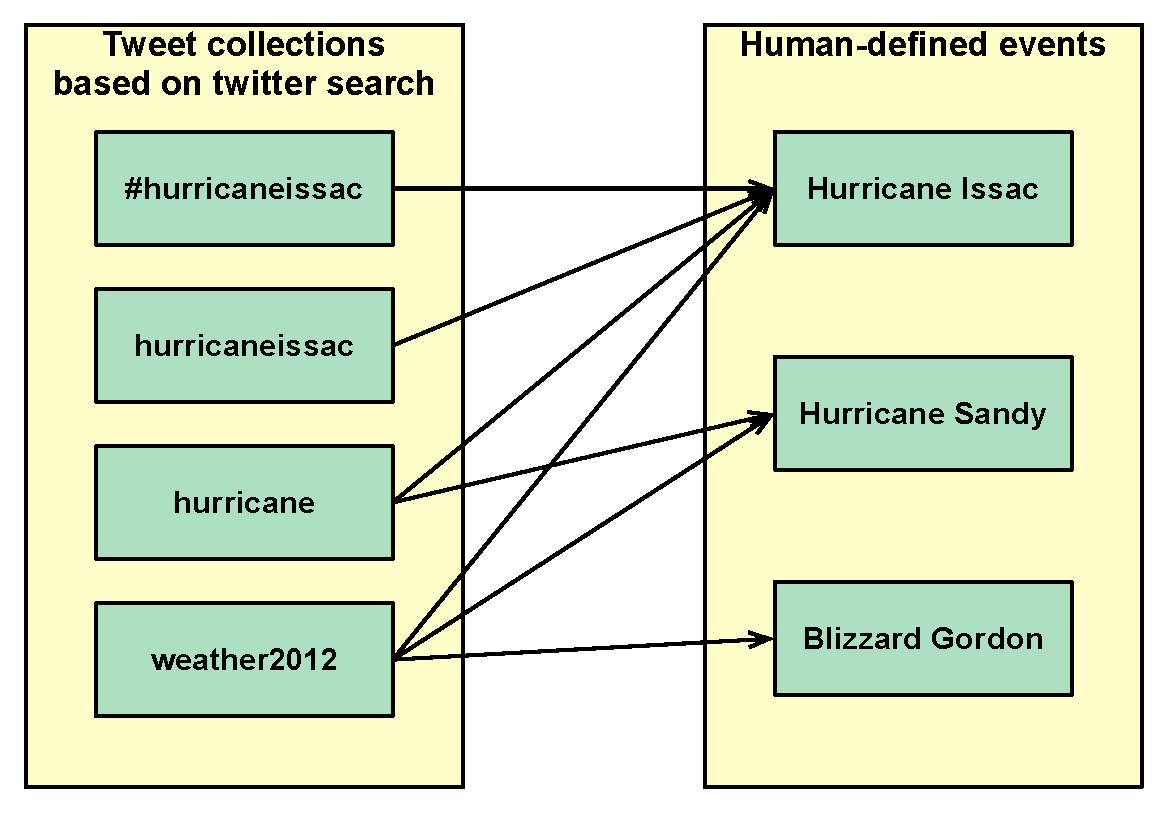
\includegraphics[width=0.5\textwidth]{figs/problem-statement.eps}
 \caption{\small Problem statement. \label{fig:statement}}
\end{figure}

\section{Requirements}
\label{sec:problemstatement}

The goal of the classification team is as follows:
 
\begin{quote}
Given a tweet collection and associated content from webpages linked in the tweets, and a set of events in the real world, we are to build a classifier that can classify the tweet and the webpages to a given event class.
\end{quote}
 
Figure~\ref{fig:statement} explains the problem  pictorially. Essentially, we have a collection of tweets  that have been retrieved based on keyword/tag search performed using the Twitter API. Additionally we have the content from webpages linked in the tweets. We will call this webpage and tweet collection together as documents in the remainder of this report, with exceptions to this convention noted explicitly. These are shown on the box on the left in Figure~\ref{fig:statement}. The human defined events or the real life events as stated in the goal are shown in the box on the right. The relationship between the collection of tweets and the events is many-to-many.

For instance, the tweet collection \fixed{weather2012} can have tweets related to the hurricanes ``Sandy'' and ``Issac'' as they occured in the same year and tweets from this collection can map to either ``Hurricane Sandy'' or ``Hurricane Issac'' event on the right. Likewise, for a given event, there can be several tweets that are associated with the event. We would also like to note that for a given event, just as there can be several tweets associated with the event, there can be multiple webpages that can be associated with the event. In a similar fashion, there could be websites that are comparing past with current events and could be classified in either event category.

For the task of classification, we make the following assumptions about the collection of tweets and webpages:
\begin{itemize}
\item Tweets have been extracted and are available as CSV files and some ``basic'' SPAM check has been done by tweet collection management team or by the teams from previous offerings of this course.
\item Webpage content will be extracted and be stripped of all tags and unrelated content by the website collection management team or by the teams from previous offerings of this course.
\item We will provide the Solr team with tweet id/webpage id and tags to classify the tweets and associated webpages.
\end{itemize}

More assumptions will be made as we make further progress on the project. We will now describe the approach that we will resort to from a very high level:

\begin{enumerate}
\item We start the process with a set of clean tweets and webpage content.
\item We perform some pre-processing to either load the data or extract only relevant parts of it.
\item Next we annotate the collection as either being relevant to a particular category or not.
\item We generate statistics related to the data obtained in step 2. 
\item The statistics are used to select features.
\item A training model is selected and using the annotated data and the set of features, its trained on.
\item This trained model is then used in classifying a larger collection of data.
\end{enumerate}

Additionally we may resort to other techniques such as bootstrap strategy to handle the larger datasets and these will become clearer in the weeks to come.

\chapter{Related Work}

We went through some papers that had done an extensive literature survey in
this field. We plan to go through the sections on comparative analysis of the
different feature selection methods described in~\cite{perira:2014:jcdl}.
We also plan to go
through the various techniques on different document representation methods
in~\cite{perira:2014:jcdl}.



\chapter{Design}
\label{chp:design}

\section{Design of the Classification System}
\label{sec:design}
 
We will use the following high level approach as shown in
Figure~\ref{fig:pipeline}.
 
\begin{itemize}
 \item {For each human defined event, we will manually identify what  tweet
collections can be used that might contain relevant tweets.}
 \item {We assume that the document collections have been cleansed of noise, SPAM and
other artifacts occurring in tweets. Some of the pre-processing of this kind
has been done by the class of Spring 2016 and saved in HBase collections. We
will use these refined collections for our work as much as possible.}
 \item {We might perform some additional noise and SPAM cleansing based on what we
observe from going through the noise/spam related artifacts from the refined
document collections.}
 \item {We will create training data out of the document collections by going though the
tweets manually and classifying them as relevant/non-relevant. To save time, we
will use the results obtained by the previous class as much as possible owing
to their availability.}
 \item {Once we have the labelled training data, we will do some statistical analysis
of the tweets based on the following techniques.}
 \begin{itemize}
  \item {Identify the top-k relevant words that correlate highly with the actual event.
Sorted TF-IDF scores.}
  \item {Top-k association rules.}
  \item {Frequent pattern mining.}
 \end{itemize}
 \item {The results of the previous step will be saved as part of the event metadata
for each human defined event. This metadata will be used to compute features
for a given tweet, during trainings, test and classification time. This
metadata will be saved in a HBase collection.}
 \item {Once we have tuned the parameters of the classifier, we will save the generated
model in HDFS. We will deploy this model in the cluster and will perform
classification on the large document collections. Please refer to Table~\ref{tbl:metadata}.}
 \item {The classified tweets will be saved back in HBase with the relevant event tags.}
\end{itemize}

\begin{figure}[t]
\centering
 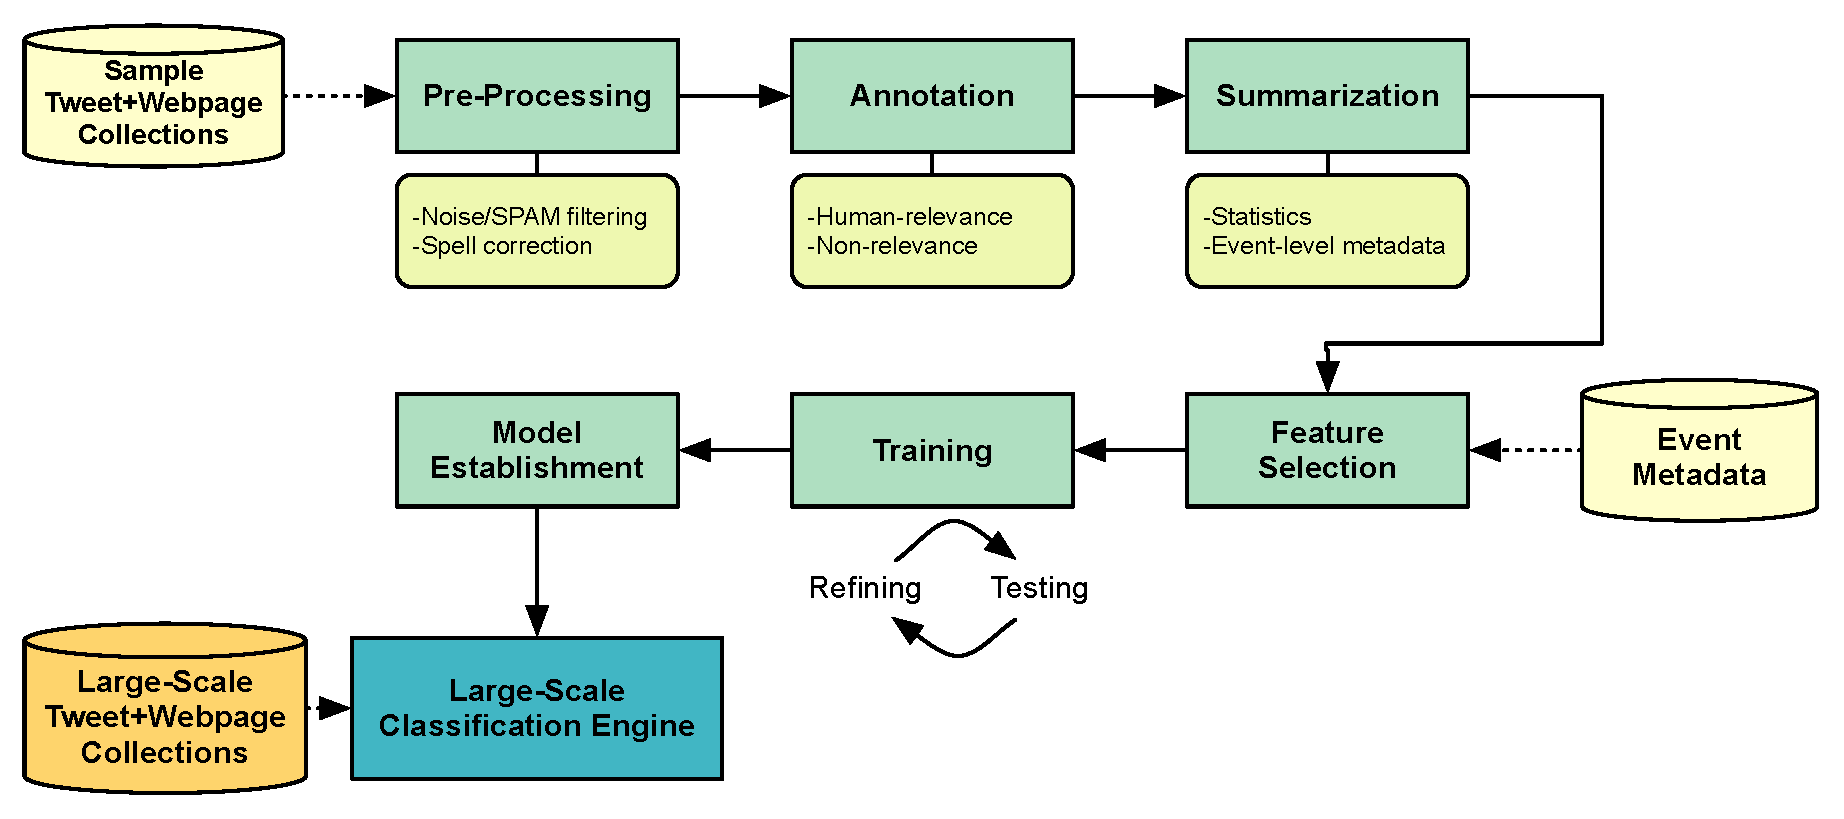
\includegraphics[width=0.9\textwidth]{figs/classification-pipeline.eps}
 \caption{\small Classification pipeline.  \label{fig:pipeline}}
\end{figure}

\begin{table}[t]
\centering
 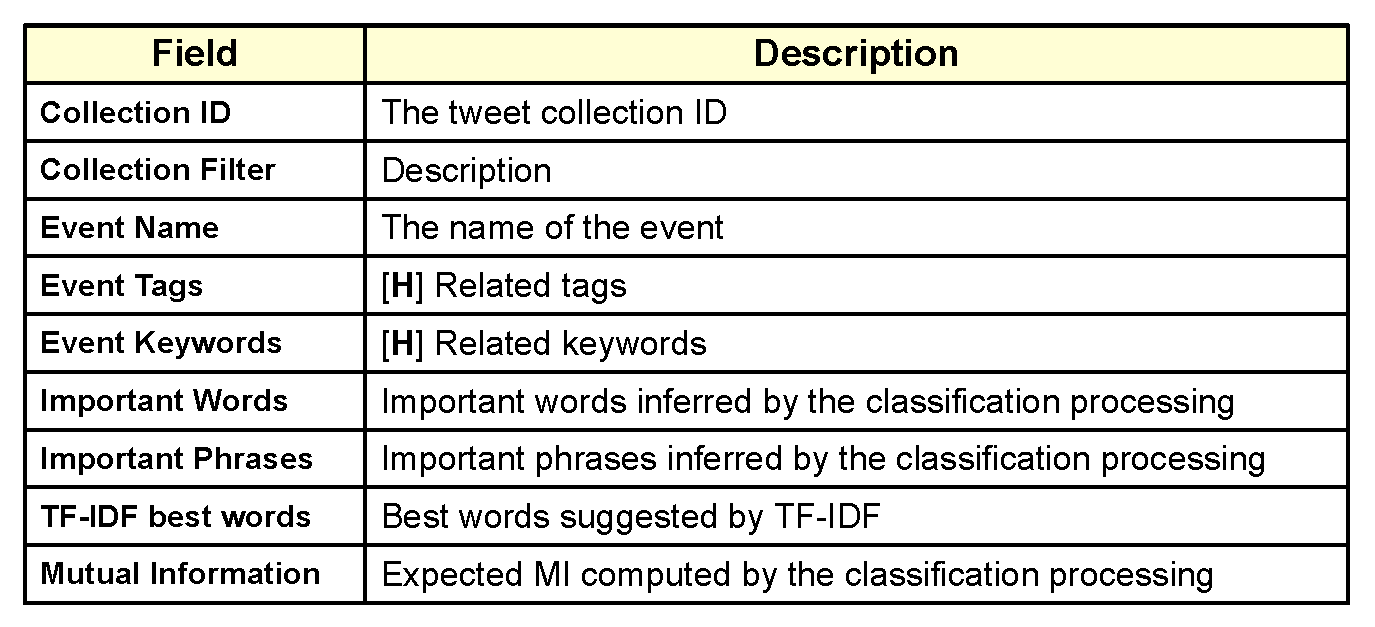
\includegraphics[width=0.8\textwidth]{figs/classmetadata.eps}
 \caption{\small Classification metadata. \label{tbl:metadata}}
\end{table}

\begin{figure}[t]
\centering
 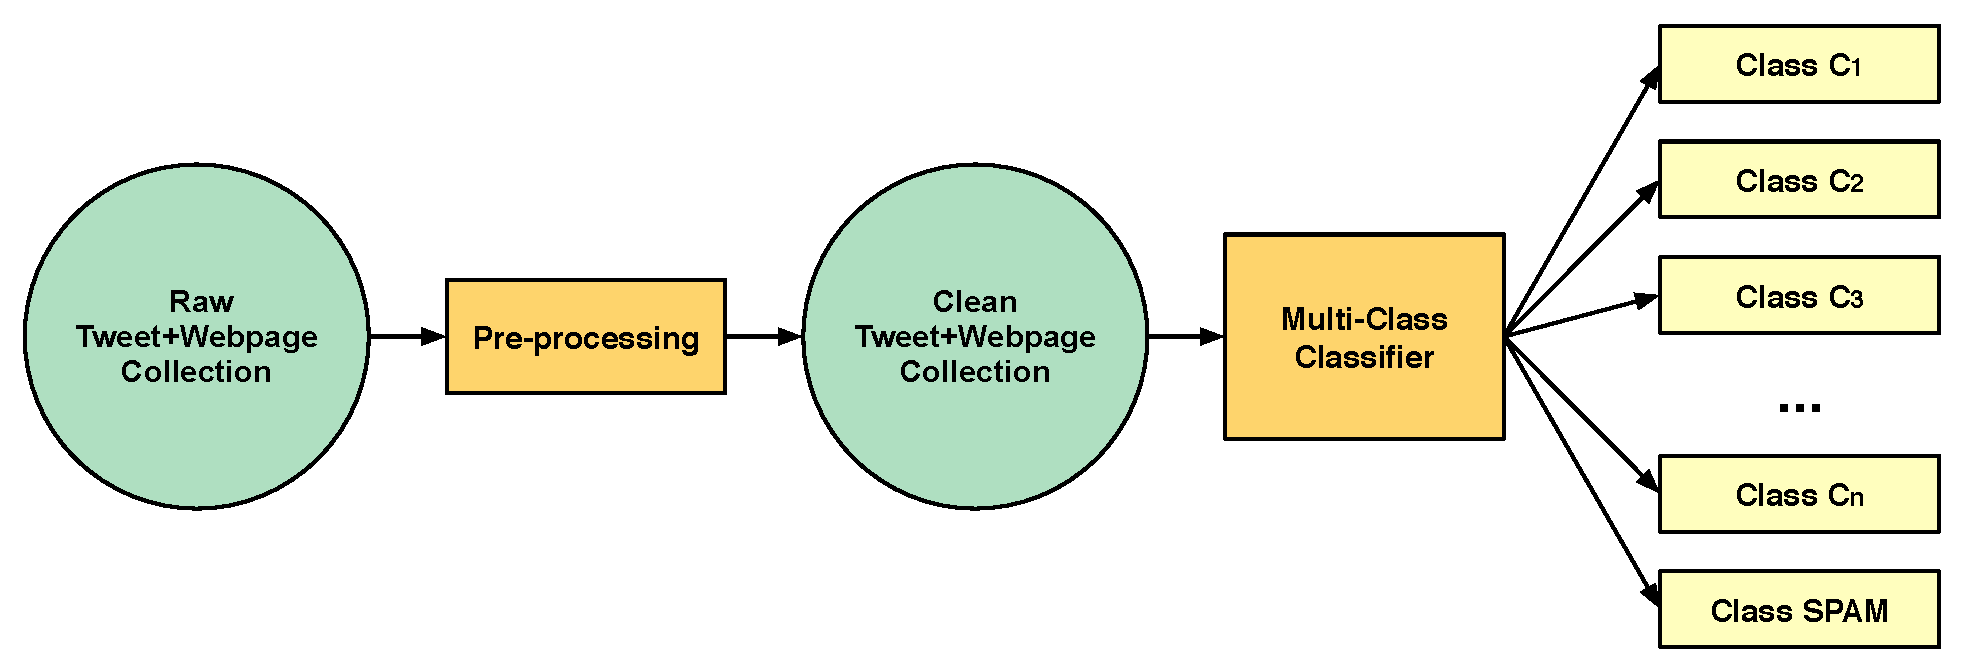
\includegraphics[width=0.9\textwidth]{figs/trainingapproach.eps}
 \caption{\small Training data approach. \label{fig:trainingapproach}}
\end{figure}



%\input{prelim}
\chapter{Execution Plan}

We plan to study the related techniques in the literature first. Then, based on
the progress, we plan to implement and evaluate our classification algorithms.


\chapter{Conclusion}

In this report, we have clarified the problem, goal, and execution plan of the
document classification team.

To summarize, we will classify the tweet and web-page collection based on the
association rule-based approach.
In addition to the algorithmic aspect, we will also try to reduce the
classification time by exploiting the benefit of in-memory data analytics
framework, e.g., Apache Spark.



%%%%%%%%%%%%%%%%%%%%%%%%%%%%%%%%

% If you are using BibTeX, uncomment the following:
%\thebibliography{refs.bib}
%
% Otherwise, uncomment the following:
%\chapter*{Bibliography}
%\settocbibname{Bibliography}
\bibliographystyle{ieeetr}
\bibliography{refs.bib}

% \appendix

% In LaTeX, each appendix is a "chapter"
% \chapter{Program Source}


\end{document}

